\chapter{Introduction}
\label{ch:intro}
\acresetall

The number of \acp{UAV} has significantly increased the last 20 years and is expected to grow more rapidly in the future. ``In the USA the number of UAVs is expected to increase from hundreds in 2015 to over 230,000 in 2035" \cite{H.Sawalmeh2018b}. The intense worldwide interest can be attributed to their reduced cost and wide range of use in applications such as search and rescue, agriculture, sea ice flow observations, inspection of infastructure, emergency communications and scientific data collection. Despite the large increase in drones, \acp{UAV} flights are permited only in secluded areas. For public areas a cumbersome authorization process is required which may take weeks or months before permission is granted \cite{Imen2016b}. In order to be granted access, it must prove its capacity to sense and safely avoid collisions with other airplanes, the ground, or other obstacles. Therefore, the need for a secure and reliable \ac{CAS} is imperative, a system that helps the drone safely navigate through an environment with obstacles.

The main role of a \ac{CAS} is to detect and predict conflicts. In case of a conflict it should perform an avoidance maneuver in order to avoid collision. However, different \acp{UAV} come with different needs and autonomy levels \cite{Albaker2009b}. How to sense the environment and gather information about the surrounding obstacles? How to detect or decide that a collision is imminent? How should the drone react when a conflict is detected? Which of the available methods show low computational cost? The answer to all these questions is what eventually defines a low-cost functional \acl{CAS}. 

In this line of reasoning, we investigate in this thesis a low computationally demanding, low-cost, vision-based, robust \acs{CAS} solution for small \acp{UAV}, primarily targeting outdoor environments. Due to time restrictions, our research targets stereo vision-based obstacle avoidance. The motivation for our choice will be clear in the following section.



\section{Problem Statement}
\label{ch:intro:problem}

A \ac{CAS} is responsible for safely navigating the drone through an environment with obstacles. A drone needs to safely and accurately avoid any surrounding threats to reach its destination. A \acs{CAS} can be divided in the following main components:

\begin{description}
	\item[Sensing:] The \textit{sensing} function defines how an \ac{UAV} acquires information about its surroundings, acknowledges obstacles and dangers that are not originally known. 
	\item[Collision avoidance:] When an imminent conflict is detected, the system has to decide how to prevent it by executing an efficient maneuver. This part can be further divided into mapping, conflict detection, path planning and dynamics.
\end{description}

The focus of this study is on a low-cost and small \acp{UAV} such as an Eachine Trashcan. Such a platform is characterized by limited computational power, power consumption and payload. For this reason, it should not make use of any dedicated hardware to accelerate the performance (e.g., FPGA or GPU) as this would increase the total cost and weight. This study assumes that the board's computational power should not exceed the one of a Cortex-A53 processor and less than 1 GB RAM should be used. These are the specifications of a low-cost platform such as a Raspberry Pi 3 Model B+ compute module (costs around 35 euros, weights 8,5 grams and consumes 1,9-2,1 Watt in idle state). 

\subsection*{Sensing}

Sensing is the first and foremost functionality of a \ac{CAS}. Over the years, a wide range of sensors have been used in obstacle avoidance such as LIDAR \cite{Xu2017} \cite{Lin2011} \cite{Scherer2008}, radar\cite{Parappat2014}, cameras \cite{Lenz2012} \cite{Lange2009} \cite{Barrientos2011a}, ultrasonic \cite{Bhardwaj2015} \cite{Gageik2012} \cite{Guerra2009} and infrared \cite{Choi2017} \cite{Gageik2015} sensors. A comparison and review of all these methods has been performed by Nyasulu, et. al \cite{DenzelNyasulu2018} which makes the following important conclusions: (1) there is no optimal sensing method, i.e., every sensor comes with its advantages and disadvantages. (2) The combination of different sensors can result in a more robust and overall increased sensing capability. With this in mind and due to timing restrictions, camera is chosen for sensing as it is a low-weight, low-cost sensor which offers a high detection range and information for the obstacle's shape. Therefore, the focus of this research is on daylight scenarios, primarily targeting an outdoor environment.

Over the years were developed many monocular, stereo and multi-camera (more than two) approaches. As the number of camera increases, the computational load and the complexity of the system increases as well \cite{Sanchez-Rodriguez2018a}. Single-camera systems are the simplest ones and because of the small dimension the camera can be easily mounted on-board. However, the state-of-the-art monocular vision methods have only demonstrated slow flights and lack reliability according to Andrew, et al \cite{Barry2018}. Multi-camera approaches take multiple photograps simultaneously to achieve 3D perception and can more easily make precise measurements as indicated by Sanchez-Rodriguez, et al \cite{Sanchez-Rodriguez2018a}. According to this study, these systems are usually more complex, most of them are fixed on the ground due to their heavy weight and high computational power is needed to process the information from the multiple cameras which cannot be mounted on board. On the other hand, stereo camera systems offer a compromise between accuracy and computational requirements and, for this reason, they have shown an increased research interest. As depicted in Figure \ref{stereo_vision_publications}, it is evident that stereo systems popularity surpasses single and multi camera approaches. 

In spite of this, there has not been found yet an optimal low-cost stereo obstacle avoidance solution. The published studies miss mainly two points: There is no up-to-date review for stereo sensing methods regarding their use in low-cost \acp{UAV} resulting in an ad-hoc decision upon the stereo algorithm to be used. Moreover, they prove their experiments by executing flights in an environment of their choice. Because of this, the imperfect accuracy of their sensing method is usually ignored. For example, in \cite{Heng2011} the flight environment is a room with some chairs in a row as obstacles. What would happen if instead of the chairs in a row there was a wide white column? Would their sensing method be able to detect it? In other words, is their sensing component of the \ac{CAS} reliable considering that an indoor environment may contain far more textureless obstacles? Another example is the study of Barry, et al \cite{Barry2018} which demonstrates successful flights in a cluttered environment. They prove their sensing method accuracy by flying in an environment with sparse trees. What would happen if the obstacle density was higher? Since there is no evaluation benchmark for \acp{CAS} taking into account the characteristics of the flight environment, this is an inherent problem of every \ac{CAS} study. In other words, the success of stereo-vision is implicitly considered as a given.

\begin{figure}[]
  \makebox[\textwidth][c]{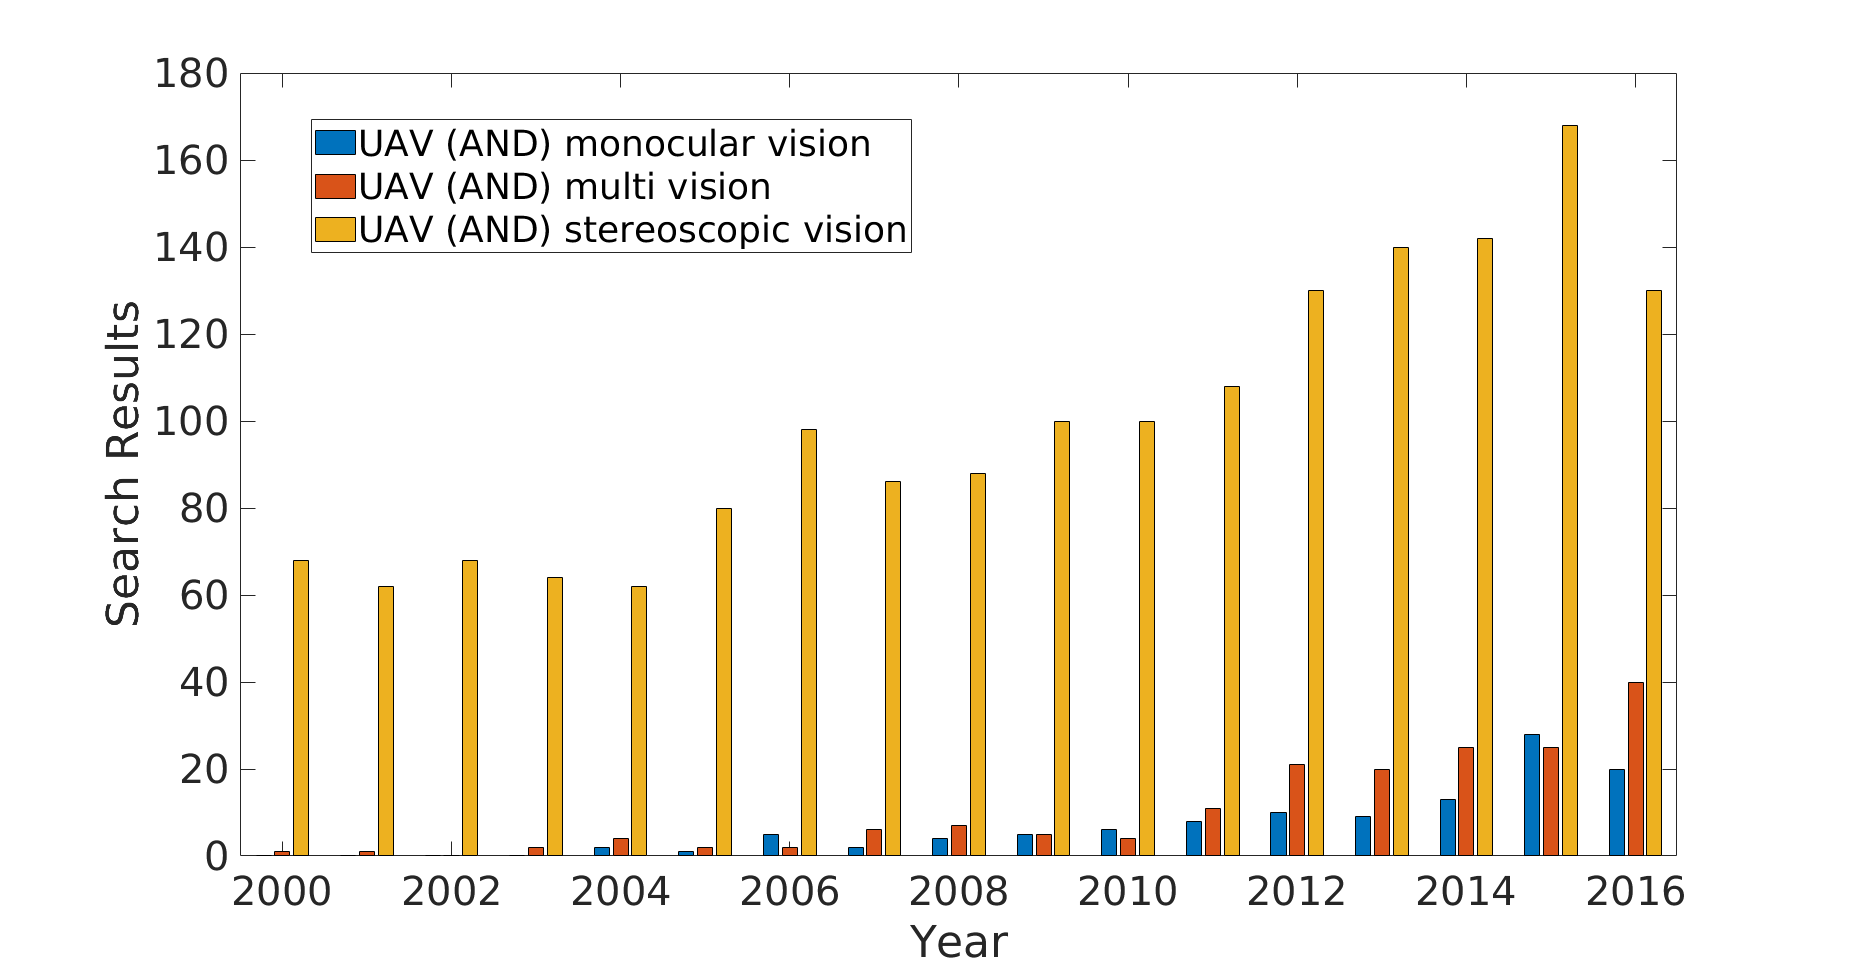
\includegraphics[width=1\textwidth]{1_introduction/images/stereo_vision_publications2.png}}
  \caption{Figure relied on information from \cite{Sanchez-Rodriguez2018a}. The Web Of Science platform was used \cite{web_of_science}}
  \label{stereo_vision_publications}
\end{figure}


\subsection*{Collision Avoidance}

In addition to its sensing ability, the \ac{CAS} includes the collision detection and avoidance part. In this research, we target static environments, therefore collision detection is simplified, and dynamics are not considered because it is is a very particular topic on its own and outside of the scope of this research. Over the last years, a large amount of mapping and path planning techniques have been developed. Most \acp{UAV} obstacle avoidance studies plan their trajectory on a discretized-space Cartesian map despite it is a very memory and resource consuming technique \cite{Brockers2016b}. Only a few studies have been conducted which significantly take into account the computational resources and perform a low-cost path planning. Moreover, most of the existing studies require accurate localization which is not necessarily needed for obstacle avoidance. A GPS system increases the cost of the overall system and low-cost products are not as much accurate as required by a \ac{CAS}. For example, a 746 GPS Breakout GPS module costs around 44 euros and has a position accuracy of $\pm$ 3 meters. Moreover, for GPS-denied environments several computer vision algorithms exist (known as Visual Odometry (VO) and Simultaneous Localization and Mapping (SLAM) algorithms) but their computational needs are way higher than a low-cost platform can afford. That said, there has not been significant development in low-cost avoidance especially without requiring the use of localization. It is true that in case the \ac{UAV} needs to autonomously reach a goal state, localization is needed and cannot be avoided. However, the focus of this research is on Collision Avoidance not autonomous navigation, therefore we assume that our system does not have localization.

\subparagraph*{Problem}

The goal of this research is to investigate stereo-based sensing and avoidance strategies and propose a collision avoidance system, assuming its use in a small, low-cost, light-weight with low-computational capacity \acs{UAV} platform, primarily targeting an outdoor environment.

\section{Research Questions}

The intense worldwide interest for safe drone flights makes the design of low-cost \ac{CAS} an imperative goal. The main result of the previous analysis is that there does not exist yet an optimal stereo-based solution for low-cost drones.

\iffalse
\begin{description}
        \item \textbf{Research goal:} Design a stereo-based low-cost Collision Avoidance System suitable for small Unmanned Air Vehicles targeting outdoor flights.
\end{description}
\fi

The first step towards the implementation of an Obstacle Avoidance Stereo-based System is to find out what stereo algorithms have been developed all these year and examine their suitability for obstacle sensing.

\begin{description}
	\item \textbf{Research question 1:} Which stereo algorithms would be good candidates for environment sensing? What criteria should be used to evaluate the existing stereo solutions?
\end{description}
	
It is very likely that existing stereo solutions present a trade-off between safely and accurately detecting the surrounding obstacle and computing time. Therefore, this trade-off should be taken into account during implementation, their errors should be analyzed and research for ways to prevent their erroneous predictions from jeopardizing the safety of our system.

\begin{description}
	\item \textbf{Research question 2:} In which way can the system overcome the erroneous depth estimations of the stereo method?
\end{description}
	
Another important part of a \ac{CAS} is the avoidance strategy to be used. A lot of different mapping and motion planning methods exist, presenting as well trade-offs between computational complexity, stored information and generated trajectories' efficiency. Since the avoidance scheme depends on the application demands, it is harder to perform an objective evaluation. Still, the existing methods should be researched and find out which one provides the best combination between accuracy and trajectory generation by taking into account its use in a small, low-cost, light-weight with low-computational capacity \acs{UAV}.

\begin{description}
	\item \textbf{Research question 3:} Which avoidance strategy should be employed considering its implementation in a small, low-cost, light-weight with low-computational capacity \acs{UAV}?
\end{description}

The answers to the above research questions will lead to the design of a \ac{CAS} suitable for small, low-cost, light-weight with low-computational capacity \acp{UAV}. Since there is not a benchmark or standard procedure to evaluate the different \ac{CAS} solutions, a comparison between this work and others is impossible. In this research, we introduce an evaluation benchmark for image-based \ac{CAS} which specifies the following criteria: the success rate of collision detection and the success rate of obstacle-free point selection. This proves the safety and reliability of the proposed \ac{CAS}.

\section{Requirements and Assumptions}

The primarily considered environment type is outdoor/textured environment. Most probably there is not an obstacle avoidance system that optimally suits both indoor and outdoor environments due to their different characteristics, flight speeds and main design problems. For example, an indoor obstacle avoidance system should focus more on the difficulty of sensing texture-less areas while an outdoor obstacle avoidance system may focus on execution time if high-speed flights are of interest. The minimum requirements and assumptions of our system are:

\begin{itemize}
	\item The loop frequency of the \ac{CAS} depends on the reaction time of \ac{UAV}, the maximum flight speed and the dynamic constraints of the model (e.g. maximum pitch acceleration, restriction in movements etc.). In this research it is assumed that the \ac{CAS} should be executed with a frequency higher than 5 Hz.
	\item The evaluation environment is outdoor and textured.
	\item The flight is supposed to take place during day-time.
	\item Only static obstacles are considered.
	\item Flights only in non-maze-like environments is assumed.
	\item The environment is considered unstructured, i.e., no information about its obstacles is available beforehand.
	\item The designed \ac{CAS} should target its application in a low-cost general purpose embedded platform such as a Raspberry Pi 3 Model B+.
	\item It should not make use of any dedicated hardware to accelerate the performance (e.g., FPGA, GPU etc.).
	\item The whole processing should be executed on-board.
	\item Localization is not available.
\end{itemize}


\section{Contributions}

During our course towards the research goal, several analysis steps have been taken. Following are the contributions:

\begin{itemize}
	\item The results show that \ac{BM} is the best and fastest solution for low-cost applications due to its low computational requirements and clear object segmentation. The main reason for rejecting \ac{ELAS} and \ac{SPS-St} is that they tend to blend the sky with foreground objects which may result in a lot of unnecessary maneuvers. In case flights in textureless environment are considered, \ac{BM} sensing performance drops a lot and \ac{SGBM} should be preferred as the second most optimal algorithm for low-cost obstacle avoidance. Profiling evaluations show that \ac{ELAS} is on average 5 times slower than \ac{BM} while \ac{SPS-St} is the slowest solution by being on average 31 times slower than \ac{BM}. On the other hand, \ac{SGBM} is not that slow as originally thought, it runs at on average $50\%$ slower than \ac{BM}.
	\item The ``uncertainty map" method was introduced and developed as a way to deal with stereo sensing inaccuracies. It is a method to estimate disparity error and the analysis show that \ac{DT} should be preferred among the candidate algorithms that could be used for this purpose. 
	\item Introduce a low-cost with low-computational capacity image-space collision avoidance which detects collisions with high accuracy and successfully generates an obstacle-free trajectory most of the time. 
	\item Implement the proposed obstacle avoidance solution and executed in real-time in a Raspberry Pi model B+.
\end{itemize}


\section{Organization}

In Chapter \ref{ch:literature} general knowledge about a \ac{CAS} is provided and the existing state-of-the-art low-cost, low-computational methods. In Chapter \ref{ch:uncertainty_map} the uncertainty map method is introduced as a way to deal with stereo sensing inaccuracies. In Chapter \ref{ch:experimental_results} the experimental setup and the experimental results are presented. Finally, in Chapter \ref{ch:conclusions} the conclusions are summed up followed by a discussion for future work.